\documentclass{standalone}

\begin{document}
\chapter*{Introduction}\addcontentsline{toc}{chapter}{Introduction}
\markboth{INTRODUCTION}{}

Colorectal cancer is a malignant neoplasm of the large intestine resulting from the uncontrolled proliferation of the cells making up the colorectal tract.
Colorectal cancer is the second malignant tumor per number of deaths after lung cancer and the third per number of new cases after breast and lung cancer\cite{cancerstats}.\\
Among the risk factors for this kind of cancer, non-hereditary ones range from colon polyps to long-standing ulcerative colitis, from Crohn's disease to old age. 
Moreover, genetic history (HNPCC or Lynch syndrome) and nutritional factors as diabetes II can increase the probability of developing cancer \cite{tesicoppola}.
Preventive measures for colorectal cancer include physical activity, reducing the consumption of processed meat and alcohol, and avoiding smoking\cite{stats2019}.
\begin{figure}[h!]
	\centering
	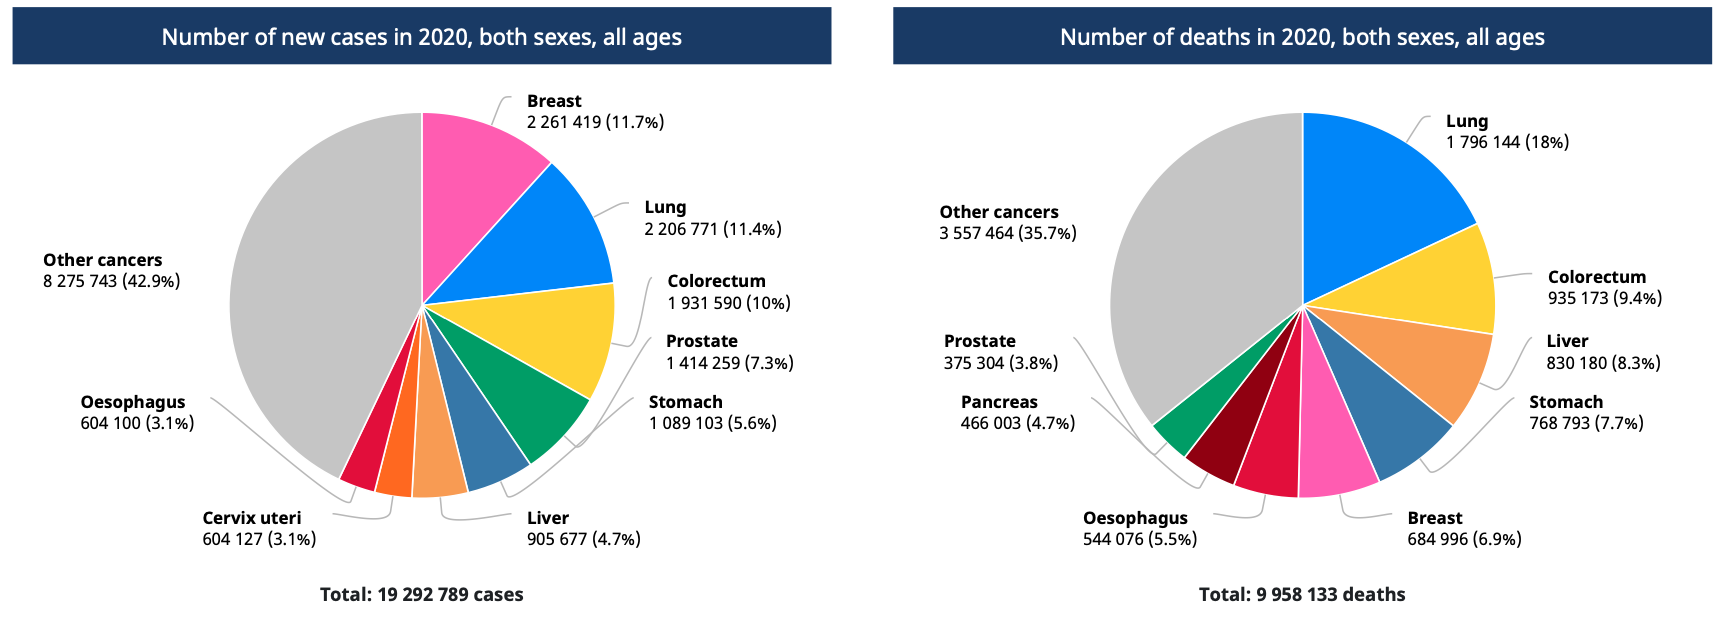
\includegraphics[width=\linewidth]{../images/cancerstats.png}
	\caption{World's cancer cases and deaths in 2020. As you can see from the \textit{Left} image, colorectal cancer is the third malignant tumor per number of new cases after breast and lung cancer while as shown on the \textit{Right} image, it is the second one per number of deaths after lung cancer. From \cite{cancerstats} }
\end{figure}
\\
Screening and diagnosis methods for colorectal cancer involve different techniques. 
The gold standard in medical routines is the colonoscopy which is an invasive technique\cite{jovana}.
Among medical imaging techniques, Magnetic Resonance Imaging (MRI) and Computed Tomography (CT) is the most used\cite{tesicoppola}. 
In particular, Magnetic Resonance Imaging (MRI) is used for pre-operative predictions and for the evaluation of the neo-adjuvant chemo-radiotherapy of patients affected by colorectal cancer\cite{tesicoppola}.

\begin{figure}[htp]

    \centering
    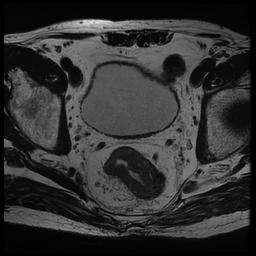
\includegraphics[width=.49\textwidth]{../images/T2AX_Alta_8.png}\hfill
    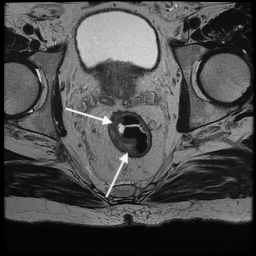
\includegraphics[width=.49\textwidth]{../images/T2AX_BO11_5.png}\hfill
    %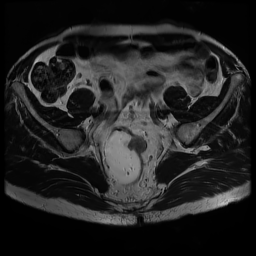
\includegraphics[width=.3\textwidth]{../images/T2AX_BO1_9.png}
    
    \caption{Magnetic Resonance images of patients affected by colorectal cancer. MRI scans can be used for pre-operative predictions and for the evaluation of the neo-adjuvant chemo-radiotherapy. From IRCCS Sant’Orsola-Malpighi Policlinic Dataset.}
    \label{trittico}
    
    \end{figure}
In order to get information about a diagnosis, therapy evaluation, stage of colorectal cancer, analysis on radiological images can be performed through the application of dedicated algorithms.\\
In this scenario, the correct and fast identification of the cancer regions is a fundamental task. 
Up to now, this segmentation task is performed using manual or semi-automatic techniques, which are time-consuming (requiring hours per day) and subjected to the operator's expertise since it requires interaction with trained specialists.\cite{tesicoppola, jovana}.
Moreover, due to the high sensitivity to the operator expertise, the obtained results cannot be reproduced\cite{Trebeschi2017}.
To overcome these issues, an automatic and fast way is required.\\
The aim of this project is to develop and implement an automated pipeline to segment MRI scans of patients affected by colorectal cancer in order to predict the response to neo-adjuvant chemo-radiotherapy. 
The work is based and tested on MRI scans provided by IRCCS Sant’Orsola-Malpighi Polyclinic.\\
The discussion will start focusing on the materials and methods: firstly, medical digital images, to understand their properties and features.
Then, an overview of the segmentation methods and the main architecture used for the identification of the cancer regions.
Also, some words about radiomics and its possible purposes.
Last but not least, an overview of Principal Component Analysis and Support Vector Classifiers will be given.
The second chapter will regard the implemented pipeline: the main description and implementation will be provided.
The obtained results will be shown and discussed in the third chapter.
Finally, the Conclusions.




\end{document}